%% note: todo's go in todo, as well as optionally in here

\section{Experiment Results}

\subsection {Methodology} 

For our experiments, we implement a prototype client in Ruby\footnote{See http://github.com/rdp/p2pwebclient} and 
run the client on members of the PlanetLab system, a pool of about 1000 servers scattered world-wide.

To run each test, a central ``driver" program contacts several of the members and instructs them to download a given file.
When peers are done downloading the file, it collects their logs and calculates conglomerate statistics.

Peers are instructed to enter the system using a Poisson distribution with an inter 
arrival time that is a total time divided by the number of peers.
For example if 1000 peers are expected to enter the system within 100s, the driver
will use a Poisson distribution with an inter arrival time of 0.1s to start up the peers, and will finish 
starting them all up at about 100 seconds.

Files are downloaded from a well provisioned server at BYU running an Apache2 web server (version 2.2.4) that is
bandwidth limited\footnote{using the mod\_bw module.} to 256 KB/s and has a 256 connection limit. 
Peers are randomly selected from available PlanetLab hosts.  If more peers download the file than
there are PlanetLab hosts available, some hosts are re-used as peers, though connections to peers on the same PlanetLab
host are disallowed.  Experiments run until 
all peers finish downloading the file. Each experiment is repeated 3 times and results are averaged. 
A different filename is downloaded with each run, so as to use ``fresh" DHT keys with each run. We collect the download 
times of all peers, and measure the amount of instantaneous load on the origin server by summing the 
bytes received from the origin per second\footnote{This only measures bytes received from the origin, not necessarily all bytes sent, 
as peers sometimes close sockets early, and any data received after a socket has already been closed is dropped by the kernel}.
We also calculate the percentage of the file received from peers and from the origin, and the times required to do DHT 
get, put, and remove operations during the course of each run, and create percentile graphs of these.  
All box plots show 25th and 75th percentiles, with outlying lines showing 1st and 99th percentiles, and middle-lines showing the median.

For default system parameters, we chose reasonable values 
of a block size of 100 KB, origin minimum speed ($R$) of 128 KB/s, $R$'s calculation window ($W$) 
of 2 seconds, and first-byte timeout ($T$) of 1 second.  Peers download the file from up to 20 other peers at a time ($b$).
Peers linger, serving the file, for 20 seconds after completing a download.

\subsection{Scaling with load}

For our first experiments we test how well our system performs under different loads.
We first test a traditional client-server transfer, to establish a base line from which to compare 
our system. Figure \ref{fig:client_server_download_times} shows the download times for client-server 
downloads, as load increases.  Median download times have a low of 1.33 seconds with a load of 1 peer/second,
and quickly grow to a high of 344 seconds with a load of 20 peers/second. Download times increase linearly instead 
of exponentially because we start a fixed number of peers and let them all complete downloads, without more peers
entering the system. 
The top outliers at a load of 20 peers/second typically wait in line about 900 seconds before 
being served the file from the origin. Load on the origin server grows quickly to its 
theoretical cap of 250 KB/s (Fig.~\ref{fig:client_server_server_load}) 
at 3 peers/second. Under a load of 20 peers/second, server speed actually decreases to 203 KB/s, which 
shows the limitations of our bandwidth limiter in that it becomes bursty and less reliable with higher connection rates. 

\begin{figure*}
  \begin{center}
    \subfigure[Load on the origin server]{
      \includegraphics[width=8.5cm]{pics/vr_unnamed316651_cs_stress_test/server_speed_Percentile_Line.pdf}
      \label{fig:client_server_server_load}
    }
    \subfigure[Download times]{
      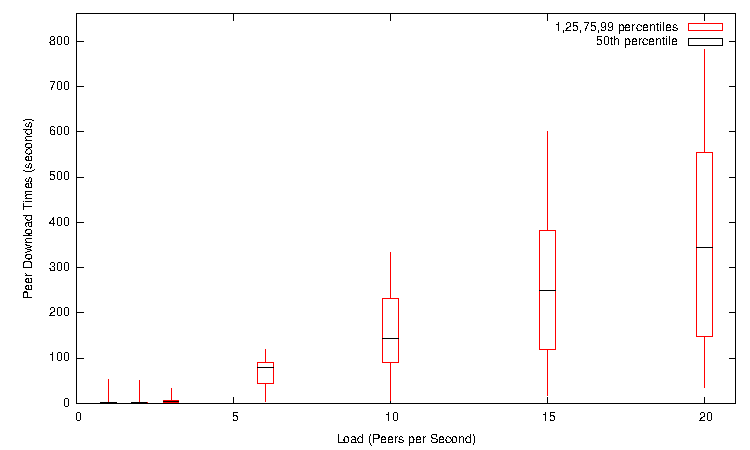
\includegraphics[width=8.5cm]{pics/vr_unnamed316651_cs_stress_test/client_download_Percentile_Line.pdf}
      \label{fig:client_server_download_times}      
    }     
    \caption{Traditional client server download}  
  \end{center}
\end{figure*}

We next test our system under the same loads. Results for download median times 
(Fig. \ref{fig:yanc_download_times}) start at 1.4 seconds at a load of 1 peer/second, and grow 
to 5.23 seconds at a load of 6 peers/s and 7.46 seconds at 20 peers/s. The graph's Y axis for download time (Fig. \ref{fig:yanc_download_times}) 
is different than that for client-server (Fig.~\ref{fig:client_server_download_times}) 
because the difference is so great that it would obscure the details. At a load of 20 peers/second 99.5\% 
of peers give up on the origin server because of a slow first byte ($T$) after one second. They then query the 
DHT for a peer list, and receive a response with a median latency of 5.215 seconds.  They download the file almost 
immediately once they receive the peer list, hence the median of about 7 seconds. 
The amount peers download from the origin decreases with higher load, mostly because Apache's bandwidth module serves 
very little when it is under high load, and also because the peers receive the file much more quickly 
from their peers and then abandon their connections to the origin (Fig. \ref{fig:yanc_origin_server_load}).

The amount of peer-to-peer transfer, as expected, increases with higher loads. Under low load peers tend to download 
the file only from the origin, however, after about 10 peers/second almost 100\% of the transfer is being 
done from peers (Fig.~\ref{fig:yanc_cdf_from_peers}--a 1 on the graph means 100\% of the file 
transfer is from peers). The reason it isn't always at 100\% for lower loads is that peers start 
downloading the file from the origin, receive some portion of it within the first $W$ (2) seconds, 
transition to peer-to-peer transfer because the rate of download is less than $R$.
The 1st percentile (fastest peers) almost always download the file directly from the origin, and are typically 
the first few peers to enter the system.  Later later peers almost always download the 
file from peers, because they encounter an already slow origin server. 

There are two basic causes for why some peers take a long time to download the file.  One is that poorly connected peers take so long to download a file 
that the peers they connect to finish lingering and drop the connection.  They then have to request a new 
list of peers from the DHT, causing an increase in latency.  This problem is exacerbated by the fact that we request 
the last block from multiple peers.  This causes 
some wasted redundancy in bytes received, which slows down incoming data, causing peers to timeout their
connections more often. The other factor causing slowdown is a sometimes unresponsive DHT. We 
set DHT requests to timeout after 60 seconds if no response is received as a reasonable value to keep from 
overloading the DHT. Typically requests come back quickly, however at times a few will timeout, 
and peers will end up downloading the entire file from the original server, or perform a new 
query after 60 seconds, and then download the file normally after that.  We're not entirely sure why this behavior occurs with Bamboo.
<%= figure_directory 'vr_medium_p2p_load_tak4', 'yanc', 'P2P results varying load' %>

\subsection{Impact of system parameters}

If a peer can download a file quickly from the origin, it does no help to download the file from its
peers. Our system accomodates for this by specifying parameters for the conditions under which it will 
transition to a peer-to-peer delivery. We test the impact of varying these and other system parameters, in order 
to explore the dynamics of our system. In each test we start 1000 peers, with an average of 15 peers entering 
the system per second, using a poisson distribution with an interarrival time of 0.066 seconds (all peers enter the system within 67 seconds). 
Peers download a 100 KB file, using the default parameters unless specified.

We first vary $T$, the timeout for a response byte from the origin server. We expect that an extremely low value 
will cause transitioning too early and an extremely high value 
will cause transitioning too late, both resulting in slow download times. Figure \ref{fig:vary_t} shows that 
the results hold to our hypothesis. With $T$ set to 0 seconds, median download time is 46.43 seconds. It then drops to 15.35 seconds with $T$ set at 0.75 seconds, 
then rises to 35 seconds with $T$ set to 10 seconds.

Fig. \ref{fig:vary_t_death_reasons} shows the break down of the reasons peers used to transition to peer-to-peer delivery.  $dT$ is the number
of peers who transition to peer-to-peer delivery because of a slow first byte, $dR$ is the number of
peers that transition because of a too low value of $R$, $died$ is the number of peers that never completed the download
(typically because their host's network access had connectivity problems) and $http\_straight$ refers to the number of peers
that download the entire file from the origin server.

A higher value of $T$ caused $R$ to become more important.  With low values of $T$, almost 100\% of peers transition to peer-to-peer delivery because of $T$. 
With $T$ at 10 seconds about 80\% of peers transition because of $T$, and 20\% because of $R$.

<%= figure_directory 'vr_unnamed17712_dT', 'vary_t', 'Varying T', true, false %>

We next examine the effect of varying $R$, the server's minimum calculated speed.  We vary $R$ from 32 KB/s to 1 MB/s, set $T$ to a 
reasonably high value of 10 seconds. The expected result us that a high value of $R$ will cause peers to transition 
too early, and that a value too low will cause peers to transition too late, both resulting in poor performance. Figure \ref{fig:vary_dr} shows that this is the case.
With $R$ set to 5 KBps, median download times are 40 seconds, with $R$ at 40 KBps, download times drop to 15 seconds, and reach
a low of 13 seconds with $R$ set to 160 KBps. Higher values than 160 KBps result in slower downloads.  $R$ set to 1 MBps has a median download time of 30 seconds. 

<%= figure_directory 'vr_unnamed502788_dR_fromStart_5000by_fixed_settingAndMajorTimes_8_times_0.0666666666666667s__10s_100000B_255000BPS_5000s_10s_2.0s_100000B', 
  'vary_dr', 'Varying R', false, false %> 

We next vary $W$, the amount of recent download time used to calculate $R$. Our hypothesis is that 
a small value for $W$ will cause the calculation to be too sensitive and unoptimal. We vary $W$ from 0.1 seconds 
to 10 seconds and run the same experiment described above with $T$ set to 10 seconds and $R$ set to 128 KB/s. Figure \ref{fig:dw} shows the results are 
slightly different than our hypothesis. Varying $W$ does make some difference, but only when set 
to a very low value. Median download times are 17 seconds with $W$ set to 0.25 seconds. For $W$ \textgreater{} 0.25 seconds
median download times stay at approximately 25 seconds. Surprisingly, 
most peers (about 800 out of 1000) still transition to peer-to-peer delivery because of 
a slow first byte ($T$), even with $T$ set to the larger value of 10 seconds. 
The reason for this is that we don't start calculating $R$ until after the first byte is received, and 
in the majority of cases (800/1000) this didn't happen until after $T$ had expired, so $T$ still 
causes most of the transitioning, and appears to be a more useful metric. A lower value of $W$ only affects the first 
200 peers, who receive bytes from the not yet overloaded origin.  These peers do transition more quickly to peer-to-peer delivery.

% ltodo so was it all the first 200 that always transition to R, so that's what sped things up a bit?

% why was this higher, then?

<%= figure_directory '837145_dw', 'dw', 'Varying W', true, false %>

\subsection{Effect for a full web page}

We next run an experiment where clients download a full web page.  The normal pattern for a page view 
is to first access some root page which references several other objects, such as images, 
javascript, flash, etc. This is the case for a 2007 snapshot of the byu.edu web site, which has a medium sized main page that 
links to over 10 other, smaller, objects.  To model this behavior, each peer first 
downloads a 100 KB file. When that file completes each peer then downloads ten 10 KB files simultaneously 
(all from the origin server), and the total time to download all 11 files is measured. We set the parameters 
to be those mentioned above for testing system parameters, and vary the load from 1 peer/second to 25 peers/second. 

The expected result for this experiment is that downloading multiple pages will be slower than downloading one 
since it will put more stress on the DHT.  Our results in Figure \ref{fig:multiple_files} prove
this hypothesis correct.  Total download time starts at 1.3 seconds, and grows quickly with higher load, approaching 
150 seconds at a load of 25 peers/second. DHT response times also grow similarly with load.  Median DHT ``put'' times start 
at 0.41 seconds at a load of 1 peer/second, and grow to 12 seconds at a load of 25 peers/second (get and remove times are similar).
This explains some of the slowdown because, since the linger time is set to 20 seconds, peer lists are outdated soon after they are created, because
they take 12 seconds to set, 12 seconds to get, and by that time the peer has already gone offline.
%Also interesting to note is the load on the origin server.  It starts at 160 KB/second, decreases to 51 KB/s at a load of 10 peers/second, 
%then increases at higher load levels than 10, because our 
%system is not able to handle the increased strain.

% todo is that what really happens though?

\begin{figure*}\begin{center} 
 \subfigure[Download times] {
  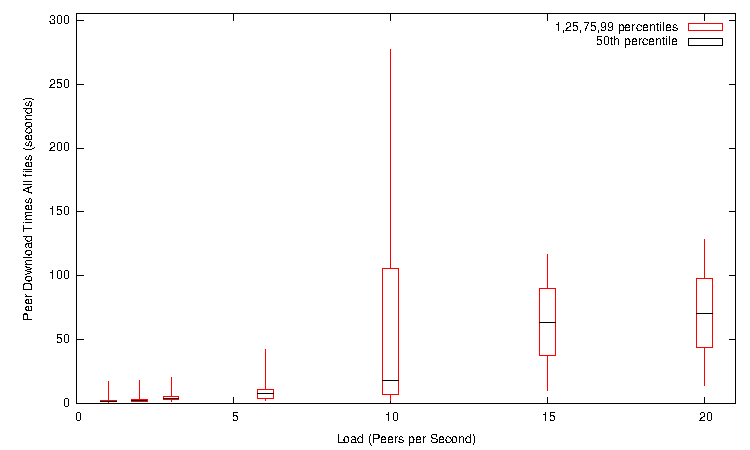
\includegraphics[width=8.5cm]{pics/vr_multiples_take_1/client_download_all_files_Percentile_Line.pdf}
  \label{fig:multiple_files_download_times_all_files}
 } 
 \subfigure[Load on the origin server] {
  \includegraphics[width=8.5cm]{pics/vr_multiples_take_1/server_speed_Percentile_Line.pdf}
  \label{fig:multiple_files_origin_server_load}
 } 
 \subfigure[Percent of file received from peers] {
  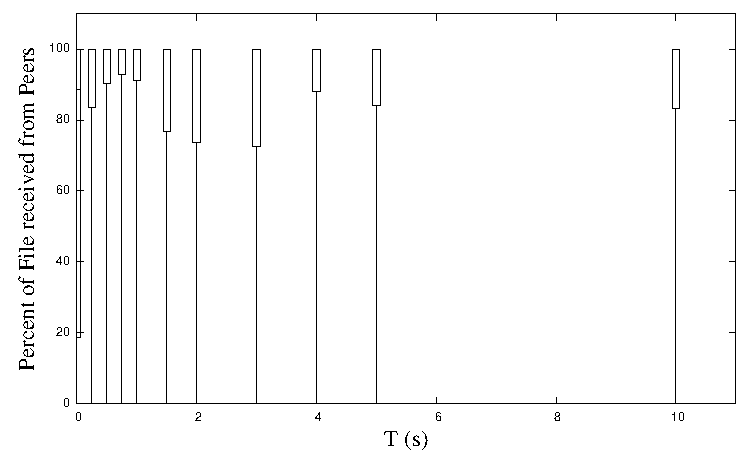
\includegraphics[width=8.5cm]{pics/vr_multiples_take_1/percent_from_clients_Percentile_Line.pdf}
  \label{fig:multiple_files_cdf_from_peers}
 }
 \subfigure[DHT put times] {
  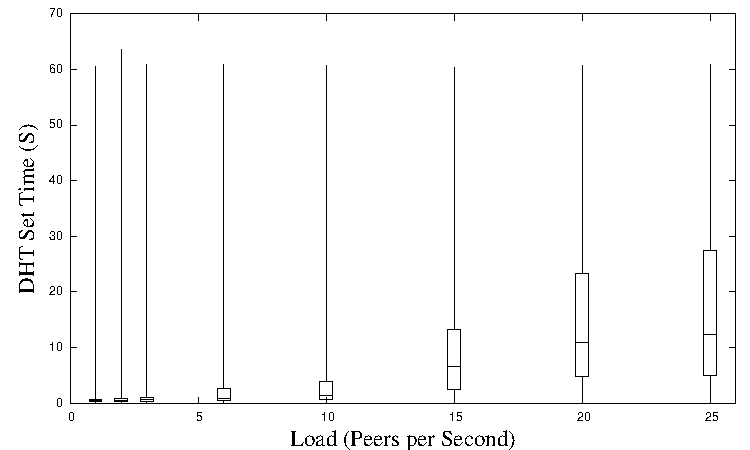
\includegraphics[width=8.5cm]{pics/vr_multiples_take_1/dht_Put_Percentile_Line.pdf}
  \label{fig:multiple_files_p2p_dht_put}
 }
 \label{fig:multiple_files}
    \caption[]{Downloading multiple simultaneous files}
    \end{center}
    \end{figure*}

As Figure \ref{fig:multiples_files_cs_download_times} shows, a client-server system still fares much worse using the same load.

<%= figure 'pics/multiples_p2p_versus_cs_pics/client_download_Percentile_Line.pdf', :caption => 'Comparison of P2P versus client server download times for multiple files', :label => 'fig:multiple_files_cs_download_times' %> 

\subsection{Varying Block Size}

We next measure the effect block size has on download time. We download a 100 KB file with block sizes ranging from 
16 KB to 100 KB, using the same default parameters as specified above for the system parameter tests.
We run 1000 peers at an average of 15 peers entering per second. Figure \ref{fig:vary_block_size} shows that 32 KB blocks result
in the quickest downloads.  This is faster because downloading more blocks allows our system to download 
several blocks from peers simultaneously.  In this case a block size of 32 KB results in a total 3 blocks, and since $b$ by default is 5, all 3 blocks
are downloaded simultaneously. 32 KB blocks were also shown to be most effective in \cite{TODO}.  

<%= figure_directory 'vr_unnamed240998_blockSize', 'vary_block_size', 'Varying block size', false, false %>

\subsection{Downloading Large Files}

We next test our system's ability to download large files. We download a 30 MB file with 100 peers, 
and then download the same file, using BitTorrent, with similar 
settings. Block size is set to 256 KB for both systems. Peers enter the system at an average of 1/s, 
and both protocols' origin servers are rate limited to 256 KB/s. For both systems, peer linger time 
is set to 0 seconds, though peers still share the file while they are downloading it. 
The expected result is that the two fare similarly. 

Our results, in Table \ref{fig:yanc_vs_bt}, show that a few peers download 
faster with our system, but most download faster with BitTorrent. 
Ours has a slower median time than BitTorrent (847 to 148 seconds), though BitTorrent has a slower time for the 99th 
percentile (2786 to 847 seconds). We're not entirely sure exactly what factors make BitTorrent faster.
We know of a few differences that could account for it.  One is that BitTorrent's seed limits its outgoing connections
to 7, whereas Apache's connection limit is 256.  This enables BitTorrent to propagate full blocks more 
quickly to peers, who then share those blocks with others.  BitTorrent seeds also favor peers who have higher download 
speeds, which helps speed propagation.  BitTorrent in this test uses a dedicated tracker, 
which makes peer rendezvous quicker than using a DHT.  It uses a ``rarest block first" policy in block 
selection, enabling it to share blocks more efficiently by sharing those that are more useful.  These differences may allow it 
to respond to a flash crowd such as this one better.  In future work we will optimize our system to handle 
flash crowds and large files, such as this one.  

One interesting statistic is the relative download speeds within each system.
The difference between 25th and 75th percentiles in our system is about 150s, 
or 5\% of the 75th percentile's time. The difference between the 25th and 75th percentiles of BitTorrent 
is 24s, or about 7\% of the 75th percentile's time. These numbers being close imply that once 
a few initial peers have downloaded a file in its entirely, it doesn't take (relatively) long infor the rest of the peers to complete 
the file a download. Figure \ref{fig:yanc_30mb_cdf} shows how much of the file that peers received from the origin.  Most comes from peer-to-peer delivery.

<%= figure 'pics/yanc_30mb/yanc_30_mb_cdf.pdf', :caption => 'CDF of percent of file received from peers, 30MB file', :label => 'fig:yanc_30mb_cdf' %>

\begin{table}
  \caption{Download times of a 30MB file}
\begin{center}
\begin{tabular}{ c c l }
  Percentiles & Our System (S) & BitTorrent (S) \\
  \hline
  1 & 613 & 131 \\
  25 & 730 & 139 \\
  50 & 847 & 148 \\
  75 & 882 & 163 \\
  99 & 982 & 2786 \\
  \label{fig:yanc_vs_bt}
\end{tabular}
\end{center}
\end{table}

\subsection{Peer connection limit b} 

We next vary the maximum number of download connections each peer is allowed at a time ($b$). We 
repeat the above 30 MB download experiment, but vary the peer connection limit from 1 to 50. 
We expect that download times will suffer if the connection limit is too low. Figure \ref{fig:vary_connection_count} shows that, as expected, median 
download times suffer when the limit is low, with a mediain download time of 1604s when the limit is 1.  Download 
times decrease with higher connection limits.  A limit of 16 has a median download time of 931s.  Limits greater than 16 don't
yield as much gain in speed. A 50 peer limit results in a median download time of 875s.

<%= figure_directory 'vr_vary_blocks_large_file', 'vary_connection_count', 'Varying number of concurrent peers', false, false %>

\section{Varying linger time}

We next vary the amount of linger time, our hypothesis being that a longer linger 
time will increase download speeds.  Figure \ref{fig:vary_linger_time} shows our hypothesis is correct.   
We download a 100K file (using the same parameters as the original system parameters test), varying linger time from 0 to 160 seconds.
With a linger time of 0 seconds, median download time was about 300 seconds, with 
a linger time of 1 second, median download time dropped to 127 seconds.  With a linger of 2 seconds, download time further dropped to 60 seconds, and
with a linger time of 4 seconds, download time dropped to 34 seconds.  Download time stays at about that level for linger times greater than 4 seconds.

<%= figure_directory 'vr_unnamed497104_linger_fromStart_0by_fixed_settingAndMajorTimes_8_times_0.0666666666666667s__0s_100000B_255000BPS_125000s_1.0s_2.0s_100000B', 
 'vary_linger_time', 'Varying linger time', false, false %> 
